\documentclass[aps,pre,amsmath,amssymb,floatfix,onecolumn,notitlepage,10pt]{revtex4-1}
\usepackage{graphicx,isomath,bm}
\usepackage[colorlinks=true,linkcolor=blue,citecolor=blue,urlcolor=blue,pdfborderstyle={/S/U/W 1}]{hyperref}

\begin{document}

\title{Dispersion and bifurcation design in viscid Faraday waves with periodic heterogeneity}
\author{Zachary G. Nicolaou}
\date{\today}

\maketitle
%\tableofcontents

\section{Introduction}
Universal pattern formation in driven and dissipative systems is dictated by wave dispersion and the development of bifurcation instabilities. The period-doubling instability of a fluid surface driven by vertical vibrations, for example, gives rise to the beautiful and fascinating Faraday wave patterns that have been studied for over a century \cite{2021_Nicolaou_1}. While universality in homogeneous systems have been thoroughly characterized, heterogeneous systems exhibit a variety of complex behaviors which are less well understood. The formation of band gaps through periodic heterogeneities, for example, is associated with the emergence of symmetry-broken localized states, leading to novel pattern-forming phenomena and potential technological applications in self-assembled systems. Recently, it was also recognized that band gaps can alter the nature of the bifurcation leading to instabilities in systems driven by vibrations through a coresonance mechanism \cite{2021_Nicolaou_2}. Rather than a single wave mode resonating with the drive to produce a response at half the driving frequency (via a period-doubling bifurcation), a pair of heterogeneity-related modes can respond with a quasiperiodic response that is incommensurate with the driving (via a Neimark-Sacker bifurcation). While coresonance can be designed in a simple system of coupled pendula with relative ease, it is unclear if this phenomena can be achieved in Faraday waves, the paradigmatic pattern-forming system driven by vibration. Here, we hope to design the dispersion and bifurcation structure in Faraday wave systems through a complete Floquet  analysis of the viscid fluid equations.

\section{Viscid fluids with periodic heterogeneity}
The incompressible Navier-Stokes equations govern the fluid motion,
\begin{align}
\rho \left(\frac{\partial \mathbf{u}}{\partial t} + (\mathbf{u}.\bm{\nabla})\mathbf{u}\right) - \mu \nabla^2 \mathbf{u} &= -\bm{\nabla}P + \rho \mathbf{g}, \label{ns} \\
\bm{\nabla} \cdot \mathbf{u} &= 0. \label{incompressible}
\end{align}
Rotational symmetry is broken by the gravitational body force, which is assumed to be oriented in the vertical direction $\hat{\mathbf{z}}$. Accordingly, we separate the lateral coordinates into a vector $\mathbf{x}=(x,y)$ and integrate out the $z$ dependence in the following. Furthermore, we take an accelerated frame of reference that moves with the vertical vibration of the container, which implies a periodic body force $\rho \mathbf{g} = \hat{\mathbf{z}}\rho (g + a_d\cos(\omega_d t))$, where $g$ is the gravitational acceleration, $a_d$ is the driving acceleration, and $\omega_d$ is the driving frequency. (Non-sinusoidal periodic driving may also eventually be of interest in order to manipulate the band structure of the response.)

The fluid-air interface is a free surface, occurring at $z=h_0 + H(\mathbf{x})$, where $h_0$ is the unperturbed fluid depth. The motion of the fluid surface is governed by a kinematic boundary condition
\begin{equation}
\left. \frac{\partial H}{\partial t} + \mathbf{u}\cdot\nabla H - \mathbf{u}\cdot\hat{\mathbf{z}} \right\rvert_{z=h_0+H} = 0. \label{kinematic}
\end{equation}
The tangential and normal  stress-balance conditions at the free interface ensure conservation of momentum,
\begin{align}
\left. 2\mu\hat{\mathbf{n}}\cdot E \cdot \hat{\mathbf{t}}_x  \right\rvert_{z=h_0+H} = 0,  \label{tangentialstress1} \\
\left. 2\mu\hat{\mathbf{n}}\cdot E \cdot \hat{\mathbf{t}}_y  \right\rvert_{z=h_0+H}  = 0, \label{tangentialstress2} \\
\left. P - 2\mu \hat{\mathbf{n}} \cdot E \cdot \hat{\mathbf{n}} - \sigma \bm{\nabla}_s \cdot \hat{\mathbf{n}}  \right\rvert_{z=h_0+H} &= 0, \label{normalstress}
\end{align}
where $\hat{\mathbf{n}}$ %= \frac{\hat{\mathbf{z}} - \hat{\mathbf{x}}\frac{\partial h}{\partial x} - \hat{\mathbf{y}}\frac{\partial h}{\partial y}}{\sqrt{1+(\frac{\partial h}{\partial x})^2+(\frac{\partial h}{\partial y})^2}}$
is the outward-pointing normal vector to the free surface, $\mathbf{t}_x$ and $\mathbf{t}_y$ are the tangential surface directions, $\sigma$ is the surface tension, $\bm{\nabla}_s$ is the surface gradient operator, and $E$ is symmetric the rate of strain tensor, with Cartesian component $E_{ij} = \frac{1}{2}\left(\frac{\partial u_{i}}{\partial x_j} + \frac{\partial u_{j}}{\partial x_i}\right)$.
Finally, there are no-slip and no-penetration boundary conditions on the fluid-solid interface, which occurs at $z=h_s(\mathbf{x})$,
\begin{equation}
\left. \mathbf{u} \right\rvert_{z=h_s} = \mathbf{0}. \label{noslip}
\end{equation}

We seek to study the linear stability of the motionless base state $\mathbf{u}_0 = \mathbf{0}$, $P_0 = \rho(g+a_d\cos(\omega_d t))z$, $H_0=0$. Let $\mathbf{u} = \mathbf{u}_0 + \bar{\mathbf{u}}$, $P=P_0+\bar{P}$, and $H=H_0+\bar{H}$, where $\bar{\mathbf{u}} = (u,v,w)$, $\bar{P}$, and $\bar{H}$ are small.  We assume that the solid interface $h_s(\mathbf{x})$ is periodic with respect to two translations, $h_s(\mathbf{x}) = h_s(\mathbf{x}+\mathbf{r}_1) = h_s(\mathbf{x}+\mathbf{r}_2)$. Given the periodicity in space and time, we know that the linearized operator that we seek will commute with the discrete space and time translation operations. This implies \cite{2006_deconinck} that we can expand the perturbations into modes using a Floquet ansatz
\begin{align}
u &= e^{i\mathbf{k}.\mathbf{x} + i\omega t}\sum_{lmn} u_{lmn}(z) e^{i(m\mathbf{k}_1\cdot \mathbf{x} + n\mathbf{k}_2\cdot \mathbf{x} + l\omega_d t)}, \label{floq1} \\
v &= e^{i\mathbf{k}.\mathbf{x} + s t}\sum_{lmn} v_{lmn}(z) e^{i(m\mathbf{k}_1\cdot \mathbf{x} + n\mathbf{k}_2\cdot \mathbf{x} + l\omega_d t)}, \label{floq2} \\
w &= e^{i\mathbf{k}.\mathbf{x} + i\omega t}\sum_{lmn} w_{lmn}(z) e^{i(m\mathbf{k}_1\cdot \mathbf{x} + n\mathbf{k}_2\cdot \mathbf{x} + l\omega_d t)}, \label{floq3} \\
\bar{P} &= e^{i\mathbf{k}.\mathbf{x} + i\omega t}\sum_{lmn} P_{lmn}(z) e^{i(m\mathbf{k}_1\cdot \mathbf{x} + n\mathbf{k}_2\cdot \mathbf{x} + l\omega_d t)}, \label{floq4} \\
\bar{H} &= e^{i\mathbf{k}.\mathbf{x} + i\omega t}\sum_{lmn} H_{lmn} e^{i(m\mathbf{k}_1\cdot \mathbf{x} + n\mathbf{k}_2\cdot \mathbf{x} + l\omega_d t)},  \label{floq5}
\end{align}
where the reciprocal lattice vectors $\mathbf{k}_i$ are defined as the dual basis to the discrete translational vectors $\mathbf{r}_j \cdot \mathbf{k}_i = 2\pi\delta_{ij}$. We aim to determine the relationship between the wavevector $\mathbf{k}$ and the (complex) response frequency $\omega$, which we refer to as the dispersion relation. (Note about the periodicity in wave vectors and frequency and the first Brillouin zones).

We now eliminate the $z$ dependence on the Floquet mode amplitudes $u_{lmn}(z)$, $v_{lmn}(z)$, $w_{lmn}(z)$, and $P_{lmn}(z)$. Note first that the advective term $\mathbf{u}\cdot\bm{\nabla}\mathbf{u}$ in Eq.~\eqref{ns} is negligible in the linear regime, since $\mathbf{u}=\bar{\mathbf{u}}$ is small. Then, taking the divergence of Eq.~\eqref{ns} and applying Eq.~\eqref{incompressible}, it follows that
\begin{equation}
\nabla^2 \bar{P}=0. \nonumber
\end{equation}
Inserting Eq.~\eqref{floq4} and projecting onto the modes (by multiplying by $e^{-i\mathbf{k}\cdot x-st-i(m'\mathbf{k}_1\cdot x+n'\mathbf{k}_2\cdot x+l'\omega_d t)}$ and integrating over the two-dimensional spatial unit cell $V$ spanned by $\mathbf{r}_1$ and $\mathbf{r}_2$), it follows that
\begin{equation}
\frac{\partial^2 P_{lmn}}{\partial z^2} - \left |\bm{\kappa}_{mn}\right|^2 P_{lmn} = 0, \nonumber
\end{equation}
where $\bm{\kappa}_{mn} = \mathbf{k} + m\mathbf{k}_1 + n\mathbf{k}_2$, and thus
\begin{equation}
P_{lmn} = A_{lmn}e^{|\bm{\kappa}_{mn}|z} + B_{lmn}e^{-|\bm{\kappa}_{mn}|z}. \label{Psol}
\end{equation}
Next, inserting Eq.~\eqref{Psol} back into Eq.~\eqref{ns} and projecting onto the modes, we find
\begin{align}
\rho\Omega_{lmn} u_{lmn} - \mu\frac{\partial ^2 u_{lmn}}{\partial z^2} &= -i\bm{\kappa}_{mn}\cdot \hat{x} (A_{lmn}e^{|\bm{\kappa}_{mn}|z} + B_{lmn}e^{-|\bm{\kappa}_{mn}|z}), \nonumber \\
\rho\Omega_{lmn} v_{lmn}  - \mu\frac{\partial ^2 v_{lmn}}{\partial z^2} &= -i\bm{\kappa}_{mn}\cdot \hat{y} (A_{lmn}e^{|\bm{\kappa}_{mn}|z} + B_{lmn}e^{-|\bm{\kappa}_{mn}|z}), \nonumber \\
\rho\Omega_{lmn} w_{lmn}  - \mu\frac{\partial ^2 w_{lmn}}{\partial z^2} &= -|\bm{\kappa}_{mn}| (A_{lmn}e^{|\bm{\kappa}_{mn}|z} - B_{lmn}e^{-|\bm{\kappa}_{mn}|z}), \nonumber
\end{align}
where $\Omega_{lmn} = i(\omega+l \omega_d) + \frac{\mu}{\rho} |\bm{\kappa}_{mn}|^2$. Thus,
\begin{align}
u_{lmn}(z) &= A^x_{lmn} e^{\sqrt{\rho\Omega_{lmn}/\mu}z} + B^x_{lmn} e^{-\sqrt{\rho\Omega_{lmn}/\mu}z} - \frac{\bm{\kappa}_{mn}\cdot \hat{x}}{\rho(\omega+l\omega_d)}(A_{lmn}e^{|\bm{\kappa}_{mn}|z} + B_{lmn}e^{-|\bm{\kappa}_{mn}|z}), \label{usol} \\
v_{lmn}(z) &= A^y_{lmn} e^{\sqrt{\rho\Omega_{lmn}/\mu}z} + B^y_{lmn} e^{-\sqrt{\rho\Omega_{lmn}/\mu}z} - \frac{\bm{\kappa}_{mn}\cdot \hat{y}}{\rho(\omega+l\omega_d)}(A_{lmn}e^{|\bm{\kappa}_{mn}|z} + B_{lmn}e^{-|\bm{\kappa}_{mn}|z}), \label{vsol} \\
w_{lmn}(z) &= A^z_{lmn} e^{\sqrt{\rho\Omega_{lmn}/\mu}z} + B^z_{lmn} e^{-\sqrt{\rho\Omega_{lmn}/\mu}z} + \frac{i|\bm{\kappa}_{mn}|}{\rho(\omega+l\omega_d)}(A_{lmn}e^{|\bm{\kappa}_{mn}|z} - B_{lmn}e^{-|\bm{\kappa}_{mn}|z}). \label{wsol}
\end{align}
To complete the solution to the bulk fluid equations, we substitute Eq.~\eqref{usol}-\eqref{wsol} into the continuity equation, leading to two constraints, since the coefficients of the exponentials depending on $z$ must vanish identically,
\begin{align}
i\bm{\kappa}_{mn}\cdot\hat{\mathbf{x}}A^x_{lmn}+i\bm{\kappa}_{mn}\cdot\hat{\mathbf{y}}A^y_{lmn}+\sqrt{\rho \Omega_{lmn}/\mu}A^z_{lmn} &= 0, \label{continuitysol1} \\
i\bm{\kappa}_{mn}\cdot\hat{\mathbf{x}}B^x_{lmn}+i\bm{\kappa}_{mn}\cdot\hat{\mathbf{y}}B^y_{lmn}-\sqrt{\rho \Omega_{lmn}/\mu}B^z_{lmn} &= 0. \label{continuitysol2}
\end{align}

We have thus eliminated the $z$ dependence from the linearized equations and are left with nine constants per mode $\bm{\xi}_{lmn}=(A_{lmn}, B_{lmn}, A^x_{lmb}, B^x_{lmb},  A^y_{lmb}, B^y_{lmb},  A^z_{lmb}, B^z_{lmb}, H_{lmn})$, which we must eliminate with the remaining equations. There are seven boundary conditions left to apply in Eq.~\eqref{noslip}-\eqref{tangentialstress2}, along with the two constraints in Eqs.~\eqref{continuitysol1}-\eqref{continuitysol2}, which form the linear system.  Denoting the $k$th component of $\bm{\xi}_{lmn}$ as $\xi_{klmn}$, we can express this system through a matrix of elements $A^{klmn}_{k'l'm'n'}(\mathbf{k}, \omega)$ as
\begin{equation}
\sum_{klmn} A^{klmn}_{k'l'm'n'}(\mathbf{k}, \omega) \xi_{klmn} = 0. \label{linear}
\end{equation}
We encode Eqs.~\eqref{continuitysol1}-\eqref{continuitysol2} for the first two sets of rows in $A^{klmn}_{k'l'm'n'}(\mathbf{k}, \omega)$ with
\begin{align}
A^{klmn}_{1l'm'n'}(\mathbf{k}, \omega) &= (i\bm{\kappa}_{mn}\cdot\hat{\mathbf{x}}\delta^{k}_{3}+i\bm{\kappa}_{mn}\cdot\hat{\mathbf{y}}\delta^{k}_{5}+\sqrt{\rho \Omega_{lmn}/\mu}\delta^{k}_{7})\delta^{lmn}_{l'm'n'}, \label{lconstraint1} \\
A^{klmn}_{2l'm'n'}(\mathbf{k}, \omega) &= (i\bm{\kappa}_{mn}\cdot\hat{\mathbf{x}}\delta^{k}_{4}+i\bm{\kappa}_{mn}\cdot\hat{\mathbf{y}}\delta^{k}_{6}-\sqrt{\rho \Omega_{lmn}/\mu}\delta^{k}_{8})\delta^{lmn}_{l'm'n'}. \label{lconstraint2}
\end{align}

We use the tangential stress balance conditions in Eqs.~\eqref{tangentialstress1}-\eqref{tangentialstress2} for the next two sets of rows. Since the symmetric rate of shear is already small,  we can use the zeroth order $\hat{\mathbf{n}}=\hat{\mathbf{z}}$, $\hat{\mathbf{t}}_x=\hat{\mathbf{x}}$, and $\hat{\mathbf{t}}_y=\hat{\mathbf{y}}$. Projecting onto the modes, we find
\begin{align}
A^{klmn}_{3l'm'n'}(\mathbf{k}, \omega) &=\Big[ e^{\sqrt{\rho\Omega_{lmn}/\mu}h_0}(\sqrt{\rho\Omega_{lmn}/\mu}\delta^k_3 + \bm{\kappa}_{mn}\cdot \hat{\mathbf{x}}\delta^k_7) + e^{-\sqrt{\rho\Omega_{lmn}/\mu}h_0}(-\sqrt{\rho\Omega_{lmn}/\mu}\delta^k_4 + \bm{\kappa}_{mn}\cdot \hat{\mathbf{x}}\delta^k_8) \nonumber \\
&\quad + 2|\bm{\kappa}_{mn}| \frac{\bm{\kappa}_{mn}\cdot \hat{\mathbf{x}}}{\rho(\omega + l \omega_d)} \left(-e^{|\bm{\kappa}_{mn}|h_0} \delta^k_1 + e^{-|\bm{\kappa}_{mn}|h_0} \delta^k_2 \right)\Big] \delta^{lmn}_{l'm'n'},   \\
A^{klmn}_{4l'm'n'}(\mathbf{k}, \omega)  &=  \Big[e^{\sqrt{\rho\Omega_{lmn}/\mu}h_0}(\sqrt{\rho\Omega_{lmn}/\mu}\delta^k_5 + \bm{\kappa}_{mn}\cdot \hat{\mathbf{y}}\delta^k_7) + e^{-\sqrt{\rho\Omega_{lmn}/\mu}h_0}(-\sqrt{\rho\Omega_{lmn}/\mu}\delta^k_6 + \bm{\kappa}_{mn}\cdot \hat{\mathbf{y}}\delta^k_8) \nonumber \\
&\quad + 2|\bm{\kappa}_{mn}| \frac{\bm{\kappa}_{mn}\cdot \hat{\mathbf{y}}}{\rho(\omega + l \omega_d)} \left(-e^{|\bm{\kappa}_{mn}|h_0} \delta^k_1 + e^{-|\bm{\kappa}_{mn}|h_0} \delta^k_2 \right)\Big] \delta^{lmn}_{l'm'n'}.
\end{align}

Next, we use the the normal stress balance condition Eq.~\eqref{normalstress} for the fifth set of row. The viscous term again follows from the zeroth order $\hat{\mathbf{n}}=\hat{z}$, while the leading order capillary term becomes $\sigma \nabla_s \cdot \hat{\mathbf{n}} = -\sigma \left(\frac{\partial^2 H}{\partial x^2}+\frac{\partial^2 H}{\partial y^2}\right)$. Since the periodic forcing term $\rho a_d \cos(\omega_d t)H$ appears in the pressure term, this equation is not diagonal in the $(l,l')$ indices,
\begin{align}
A^{klmn}_{5l'm'n'}(\mathbf{k}, \omega) &= \Big[ -\rho (g+\sigma|\bm{\kappa}_{nm}|^2)\delta^k_9 + \left(\rho+\frac{2\mu|\bm{\kappa}_{nm}|^2}{i\rho(\omega+l\omega_d)}\right)\left(e^{|\bm{\kappa}_{nm}|h_0}\delta^k_1 + e^{-|\bm{\kappa}_{nm}|h_0}\delta^k_2 \right) \nonumber \\
&\quad - 2\mu/\rho\sqrt{\rho\Omega_{lmn}/\mu}\left(e^{\sqrt{\rho\Omega_{lmn}/\mu}h_0}\delta^k_7 - e^{-\sqrt{\rho\Omega_{lmn}/\mu}h_0}\delta^k_8\right)\Big]\delta^{mnl}_{m'n'l'}-\rho a_d \delta^k_9 (\delta^l_{l'+1}+\delta^l_{l'-1})\delta^{mn}_{m'n'}/2.
\end{align}

We use the kinematic boundary condition Eq.~\eqref{kinematic} for the sixth set of rows, noting that $\mathbf{u}\cdot\nabla H$ can be neglected and projecting onto the modes
\begin{align}
A^{klmn}_{6l'm'n'}(\mathbf{k}, \omega) = \left[i(\omega+l\omega_d)\delta^k_9 - e^{\sqrt{\rho\Omega_{lmn}/\mu}h_0}\delta^k_7 - e^{-\sqrt{\rho\Omega_{lmn}/\mu}h_0} \delta^k_8 - \frac{i|\bm{\kappa}_{mn}|}{\rho(\omega+l\omega_d)}(e^{|\bm{\kappa}_{mn}|h_0}\delta^k_1 - e^{-|\bm{\kappa}_{mn}|h_0}\delta^k_2)\right]\delta^{lmn}_{l'm'n'}. \label{lkinematic}
\end{align}

The final three rows will follow from the no-slip and no-penetration conditions at the solid-liquid interface, Eq.~\eqref{noslip}. Unlike the first six rows, the heterogeneity in the substrate shape $h_s(\mathbf{x})$ means that the linearized equations will not be diagonal in the spatial indices $(n,n')$ and $(m,m')$. In order to project the equations onto the Floquet basis, we need to evaluate integrals $I_{m-m'\, n-n'} =\int_V e^{i(m-m')\mathbf{k}_1\cdot\mathbf{x}+i(n-n')\mathbf{k}_2\cdot\mathbf{x}}e^{\alpha h_s(\mathbf{x})} d^2x$, where $V$ is the unit cell spanned by the spatial periodicity vectors $\mathbf{r}_1$ and $\mathbf{r}_2$. Let us assume, for simplicity, that $h_s(\mathbf{x}) = a_s(f(\mathbf{k}_1\cdot x)+f(\mathbf{k}_2\cdot x))/2$, where $f$ is a $2\pi$-periodic function and $a_s$ is a parameter describing the substrate height. In this case, the relevant integral factorizes as $I_{m-m'\, n-n'}  = I_{m-m'}(\alpha a_s/2)I_{n-n'}(\alpha a_s/2)$, where $I_{m}(\alpha a_s/2)=\int_0^{2\pi} e^{im\lambda+\alpha a_s f(\lambda)/2} d\lambda$. When $f(\lambda)=\sin(\lambda)$, for example, the $I_{m}(\alpha a_s/2)$ is the modified Bessel function. Then, projecting Eq.~\eqref{noslip} onto the modes gives
\begin{align}
A^{klmn}_{7l'm'n'}(\mathbf{k}, \omega) &= \Big[ \delta^k_{3} I_{m-m'\, n-n'} (\sqrt{\rho\Omega_{lmn}/\mu}a_s/2)  + \delta^k_{4} I_{m-m'\, n-n'} (-\sqrt{\rho\Omega_{lmn}/\mu}a_s/2) \label{lnoslip1}  \nonumber  \\
&\quad - \frac{\bm{\kappa}_{mn}\cdot \hat{x}}{\rho(\omega+l\omega_d)}(\delta^k_{1} I_{m-m'\, n-n'} (|\bm{\kappa}_{mn}|a_s/2) + \delta^k_{2} I_{m-m'\, n-n'} (-|\bm{\kappa}_{mn}|a_s/2) \Big]\delta^l_{l'},  \\
A^{klmn}_{8l'm'n'}(\mathbf{k}, \omega) &= \Big[ \delta^k_{5} I_{m-m'\, n-n'} (\sqrt{\rho\Omega_{lmn}/\mu}a_s/2)  + \delta^k_{6} I_{m-m'\, n-n'} (-\sqrt{\rho\Omega_{lmn}/\mu}a_s/2)  \nonumber \\
&\quad - \frac{\bm{\kappa}_{mn}\cdot \hat{y}}{\rho(\omega+l\omega_d)}(\delta^k_{1} I_{m-m'\, n-n'} (|\bm{\kappa}_{mn}|a_s/2) + \delta^k_{2} I_{m-m'\, n-n'} (-|\bm{\kappa}_{mn}|a_s/2) \Big]\delta^l_{l'},   \label{lnoslip2} \\
A^{klmn}_{9l'm'n'}(\mathbf{k}, \omega) &= \Big[ \delta^k_{7} I_{m-m'\, n-n'} (\sqrt{\rho\Omega_{lmn}/\mu}a_s/2)  + \delta^k_{8} I_{m-m'\, n-n'} (-\sqrt{\rho\Omega_{lmn}/\mu}a_s/2) \nonumber \\
&\quad + \frac{i|\bm{\kappa}_{mn}|}{\rho(\omega+l\omega_d)}(\delta^k_{1} I_{m-m'\, n-n'} (|\bm{\kappa}_{mn}|a_s/2) - \delta^k_{2} I_{m-m'\, n-n'} (-|\bm{\kappa}_{mn}|a_s/2) \Big]\delta^l_{l'}. \label{lnoslip3}
\end{align}
(There may be incorrect factors of $i$ and $-1$ in the modified Bessel function here...)

While Eqs.~\eqref{linear}-\eqref{lnoslip3} form a closed linear system, it is helpful to reduce the dimension of the problem by taking advantage of the partial diagonality of some of the equations.  In fact, we can eliminate the variables $\bm{\zeta}_{lmn}=(A_{lmn},B_{lmn},A^x_{lmn},A^y_{lmn},A^z_{lmn},B^z_{lmn})$ in favor of $\bm{\eta}_{lmn}=(B^x_{lmn},B^y_{lmn},H_{lmn})$ by rearranging the equations into a block matrix form
\begin{equation}
\sum_{lmn} \begin{pmatrix} A\delta^{lmn}_{l'm'n'}(\mathbf{k},\omega) & B^{lmn}_{l'm'n'}(\mathbf{k},\omega) \\ C^{lmn}_{l'm'n'}(\mathbf{k},\omega) & D^{lmn}_{l'm'n'}(\mathbf{k},\omega) \end{pmatrix} \cdot \begin{pmatrix} \bm{\zeta}_{lmn} \\ \bm{\eta}_{lmn}\end{pmatrix} = 0,
\end{equation}
where Eqs.~\eqref{lconstraint1}-\eqref{lkinematic} correspond to the first block row and Eqs.~\eqref{lnoslip1}-\eqref{lnoslip3} correspond to the second block row, and we have already factored the top left block into a diagonal part and a $6\times 6$ block matrix $A$.  (It is not possible to eliminate all combinations of $6$ variables, since the matrix $A$ may be singular for certain combinations. The specific choice here involving $\bm{\zeta}_{lmn}$ seems to be more numerically stable than other options, but may not be optimal.) This factorization makes the inversion of the first block row possible, leading to $\bm{\zeta}_{l'm'n'} =- \sum_{lmn} A^{-1} B^{lmn}_{l'm'n'}\bm{\eta}_{lmn}$, which can be substituted back into the last block row to give
\begin{align}
\sum_{lmn} E_{l'm'n'}^{lmn}(\mathbf{k},\omega) \bm{\eta}_{lmn} = 0, \text{ where } E_{l'm'n'}^{lmn} \equiv D^{lmn}_{l'm'n'} - \sum_{l''m''n''} C^{lmn}_{l''m''n''}A^{-1}B^{l''m''n''}_{l'm'n'}. \label{neigen}
\end{align}
This is the furthest possible trivial reduction since the remaining equations are not diagonal with respect to any of the indices. (It remains to correctly write down the matrix elements $E^{lmn}_{l'm'n'}$ so that it can be numerically computed).

Nontrivial solutions to Eq.~\eqref{neigen} only exist for special values of $\omega$ and $\mathbf{k}$ for which $\det E_{l'm'n'}^{lmn}(\mathbf{k},\omega)=0$, and such values define the dispersion relation that we seek. However, unlike the usual linear eigenvalue problem, Eq.~\eqref{neigen} has a complicated, nonlinear dependence on $\mathbf{k}$ and $\omega$. Unfortunately, global algorithms to find all eigenvalues for such nonlinear eigenvalue problem are not available. Iterative algorithms such as the Raleigh quotient iteration described below can identify eigenvalues given a sufficiently good initial approximation. We thus hope to numerically continue the dispersion relation starting from the inviscid limit, in which the problem reduces to a linear one, as detailed next.

\section{The inviscid limit}
In the inviscid ($\mu=0$) limit of Eq.~\eqref{ns}, the highest order spatial derivatives vanish. Thus, small viscosity is a singular perturbation of the inviscid limit, and we expect to find fewer integration constants and eigenmodes in the inviscid case (the missing modes are assumed to be evanescent and represent viscous boundary layer effects, but may become relevant in certain conditions). In fact, the inviscid velocity solution that is analogous to Eqs.~\eqref{usol}-\eqref{wsol} does not include the terms involving $(A_{lmn}^x,B_{lmn}^x,A_{lmn}^y,B_{lmn}^y, A_{lmn}^z, B_{lmn}^z)$. Correspondingly, the additional continuity constraints in Eqs.~\eqref{continuitysol1}-\eqref{continuitysol2}, the tangential stress balance conditions in Eqs.~\eqref{tangentialstress1}-\eqref{tangentialstress2}, and the tangential components of Eqs.~\eqref{noslip} representing the no-slip condition are not included in the problem. Incidentally, it follows that the solution is irrotational and the analysis can be expressed in terms of the Bernoulli equation, as was done in \cite{2021_Nicolaou_1} for a one-dimensional surface. The two-dimensional problem can also be carried out without significant changes. For the undriven case with $a_d=0$, the system reduces to a simpler generalized eigenvalue problem,
\begin{equation}
\sum_{mn} C^{mn}_{m'n'} H_{mn} = \omega^2 \sum_{mn} D^{mn}_{m'n'}, H_{mn}
\end{equation}
where
\begin{align}
C^{m'n'}_{mn}&=\left| \bm{\kappa}_{mn}\right| \left(\frac{\sigma  \left| \bm{\kappa}_{mn}\right| ^2}{\rho }+g\right) \left(e^{-{h_0} \left| \bm{\kappa}_{mn}\right| } I_{m-m'\, n-n'}\left(\left| \bm{\kappa}_{mn}\right|  {a_s}/2\right) + e^{{h_0} \left| \bm{\kappa}_{mn}\right| } I_{m-m'\, n-n'}\left(-\left| \bm{\kappa}_{mn}\right|  {a_s}/2\right) \right) \nonumber \\
&\quad \times \left(1- \left(\frac{({n}-{n'}) \bm{\kappa}_{mn}.\mathbf{k}_1}{\left| \bm{\kappa}_{mn}\right| ^2}+\frac{({m}-{m'}) \bm{\kappa}_{mn}.\mathbf{k}_2}{\left| \bm{\kappa}_{mn}\right| ^2}\right)\right), \\
D^{m'n'}_{mn}&= \left(e^{-{h_0} \left| \bm{\kappa}_{mn}\right| } I_{m-m'\, n-n'}\left(\left| \bm{\kappa}_{mn}\right|  {a_s}/2\right) - e^{{h_0} \left| \bm{\kappa}_{mn}\right| } I_{m-m'\, n-n'}\left(-\left| \bm{\kappa}_{mn}\right|  {a_s}/2\right) \right) \nonumber \\
&\quad \times \left(1- \left(\frac{({n}-{n'}) \bm{\kappa}_{mn}.\mathbf{k}_1}{\left| \bm{\kappa}_{mn}\right| ^2}+\frac{({m}-{m'}) \bm{\kappa}_{mn}.\mathbf{k}_2}{\left| \bm{\kappa}_{mn}\right| ^2}\right)\right).
\end{align}
The problem is a quadratic eigenvalue problem in the driven case, but it suffices to start from the simpler undriven case here since we can numerically continue with respect to both the viscosity and the driving amplitude, as decribed below. An example dispersion relation for an inviscid fluid on a hexagonal and sinusoidal substrate is shown in Fig.~\ref{fig1}.
\begin{figure}[hbt]
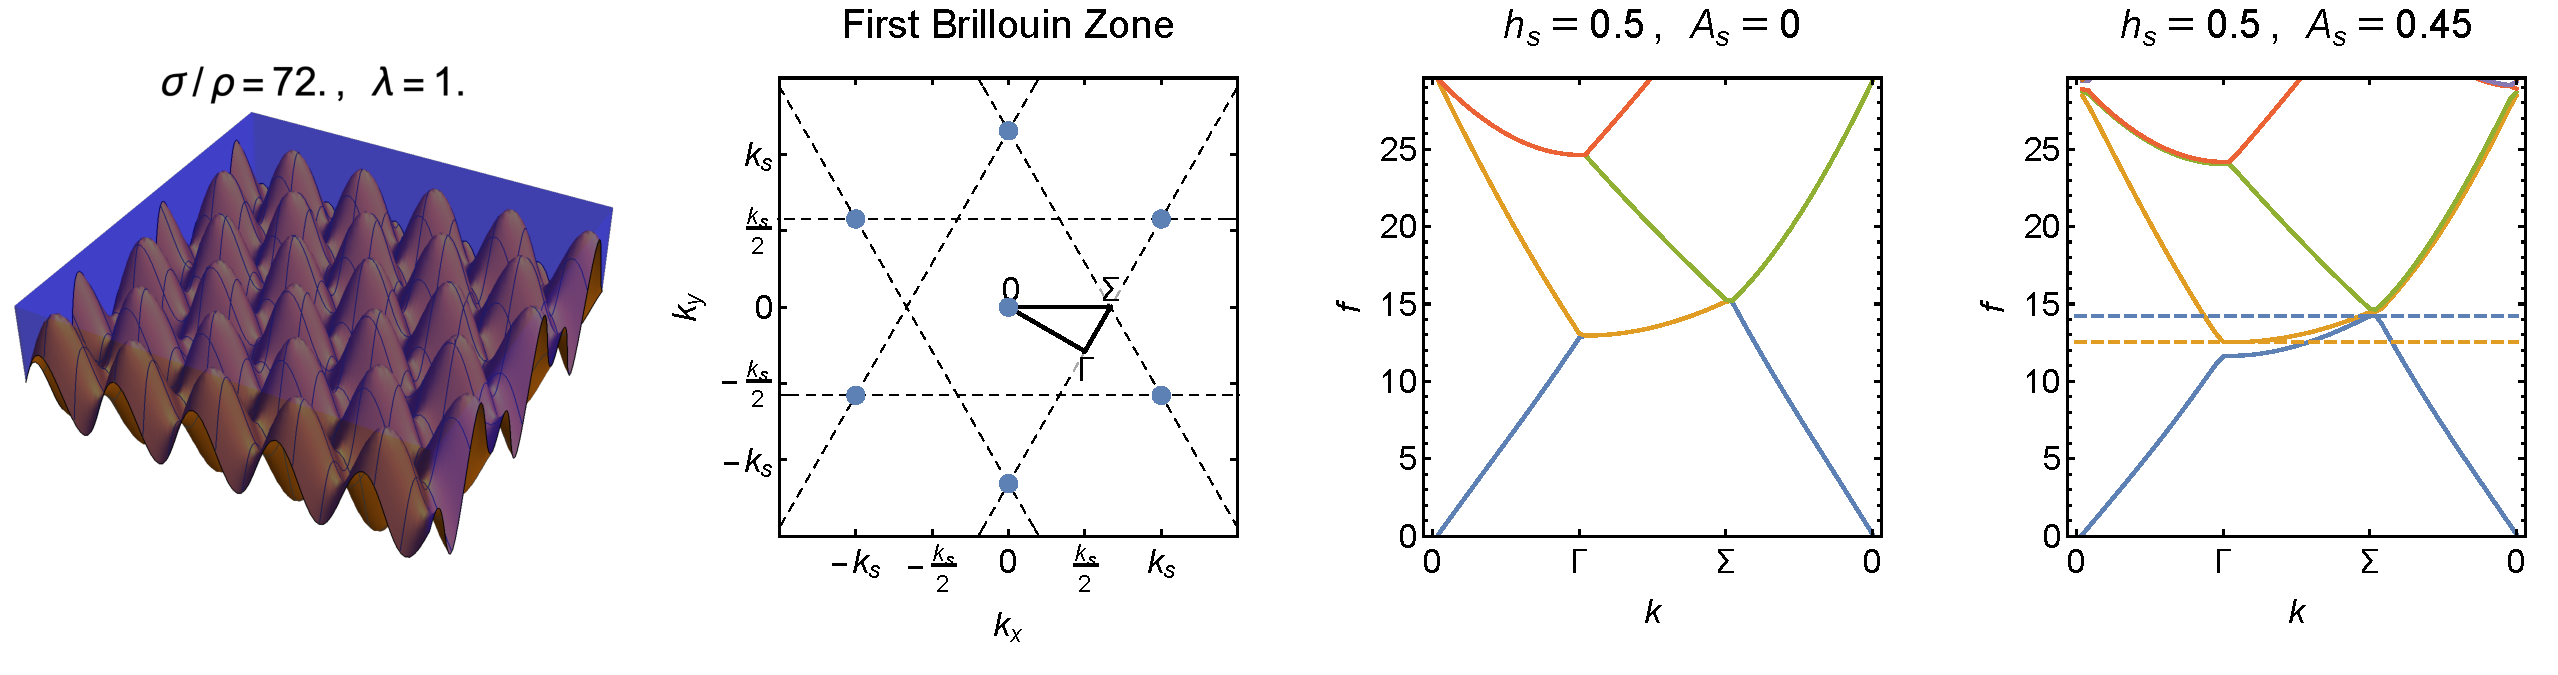
\includegraphics[width=\columnwidth]{hexagonal}
\caption{Inviscid dispersion relation for a hexagonal lattice. \label{fig1}}
\end{figure}

\section{Nonlinear eigenvalue continuation}
Consider a nonlinear eigenvalue problem
\begin{equation}
T(\lambda) \mathbf{v} = 0,
\end{equation}
where we seek values of $\lambda$ such that $\det T(\lambda)=0$, so that nontrivial solutions exist. Consider values of $\lambda=\lambda_0$ close to an eigenvalue, along with an initial approximations $\mathbf{v}_0$ and $\mathbf{w}_0$ for the corresponding left and right eigenvectors. Linearizing around $(\lambda-\lambda_0)$ and neglecting higher order terms, we find the linear generalized eigenvalue problem
\begin{align}
(T(\lambda_0)-\lambda_0 T'(\lambda_0))\mathbf{v} = -\lambda T'(\lambda_0) \mathbf{v}, \\
(T(\lambda_0)-\lambda_0 T'(\lambda_0))^\dagger \mathbf{w} = -\lambda^* T'(\lambda_0)^\dagger \mathbf{w}.
\end{align}
Given good initial guesses, the Rayleigh quotient iteration converges quadratically to the true eigenvalue \cite{1973_Ruhe}. This eigenvalue estimate is first updated using the Raleigh quotient from the current estimates, which gives  the updated estimate $\lambda_{n+1} = \lambda_n - \mathbf{w}^\dagger T(\lambda_n) \mathbf{v} /  \mathbf{w}^\dagger T'(\lambda_n) \mathbf{v}$. Since the spectrum of the inverse matrix $T(\lambda)^{-1}$ will be dominated by the corresponding inverse eigenvalue, repeated action of $T(\lambda)^{-1}$ will converge to the eigenvectors of interest. This underlies the inverse power component of the iteration, in which the eigenvector estimates are updated by solving the systems of linear equations $T(\lambda_n) \mathbf{v}_{n+1} = T'(\lambda_n)\mathbf{v}_n$ and $T(\lambda_n)^\dagger \mathbf{w}_{n+1} = T'(\lambda_n)^\dagger \mathbf{w}_n$ (and normalizing between iterations). 

By slowly varying the viscosity and the driving amplitude and applying the Rayleigh quotient iteration, we can then hope to numerically continue the inviscid and undriven dispersion relation to discover the bifurcations leading to the instabilities in the viscous system. One challenge that will arise is that eigenvalues will become degenerate during the continuation, as is known to correspond to the onset of resonance and coresonance in the pendulum system in \cite{2021_Nicolaou_2}. It may therefore be necessary to generalize the nonlinear Rayleigh quotient iteration to a nonlinear Arnoldi iteration. 

\begin{thebibliography}{99}
\bibitem{2021_Nicolaou_1} Z. G. Nicolaou, D. J. Case, E. B. Van der Wee, M. M. Driscoll, and A. E. Motter. Heterogeneity-stabilized homogeneous states in driven media. \textit{Nature communications} \textbf{12}, 4486 (2021).
\bibitem{2021_Nicolaou_2} Z. G. Nicolaou and A. E. Motter. Anharmonic classical time crystals: A coresonance pattern formation mechanism. \textit{Physical Review Research} \textbf{3}, 023106 (2021).
\bibitem{2006_deconinck}B. Deconinck and J. N. Kutz. Computing spectra of linear operators using the Floquet–Fourier–Hill method. Journal of Computational Physics \textbf{219}, 296-321 (2006).
\bibitem{1973_Ruhe} A. Ruhe, Algorithms for the nonlinear eigenvalue problem. SIAM Journal on Numerical Analysis, \textbf{10},674-689 (1973).
\end{thebibliography}
\end{document}
